% vim: set spelllang=fr:
\setchapterpreamble[ur][.7\textwidth]{%
  \dictum[Robin Hobb, \textit{La Voie magique}]{%
      Je levai les yeux vers leurs visages effrayés et me rendit compte qu'ils parlaient -- non, ils hurlaient presque ; [...] quelqu'un demandait sans cesse : « Que s'est-il passé ? Que s'est-il passé ? » Je fus soudain frappé du manque de grâce de la parole : tous ces mots rattachés les uns aux autres, que chaque bouche prononçait différemment... Et c'était ainsi que nous communiquions ?}}
\chapter{\verbenet{} : une traduction de VerbNet}
\label{ch:verbnet}

La ressource VerbNet (section~\ref{presentation_verbnet}) rend possible
l'annotation en rôles sémantiques selon nos objectifs présentés à la
section~\ref{objectifs_these}. Or, nous désirons réaliser cette annotation en
français mais VerbNet n'est disponible que pour l'anglais. C'est pourquoi nous
présentons dans ce chapitre sa traduction vers le français, nommée
\verbenet{}\footnote{Le nom vient de la prononciation à la française qui
    "rajoute" un \textit{e}. Le $\ni$ est là pour bien marquer ce \textit{e} et
ainsi essayer d'éviter la confusion avec VerbNet.}. Une partie conséquente de
ce chapitre provient d'articles déjà publiés
\citep{danlos2014vers,pradet2014adapting}. Nous avons réalisé la première étape
de traduction en collaboration avec Laurence Danlos. Ensuite, Laurence Danlos
et Takuya Nakamura ont réalisé seuls le travail lexicographique, c'est-à-dire
les deuxième et troisième étapes. Pour faciliter ce travail, nous avons
développé et activement maintenu une interface d'édition entièrement pensée
pour VerbNet afin de faciliter le travail lexicographique
(section~\ref{toolquentin}).

Ce travail a été rendu possible par une interface
d'édition développée par nos soins rendant l'édition facile afin que les
lexicographes puissent se concentrer sur le 

La construction de cette ressource se fait en trois étapes.
\begin{enumerate}
    \item Nous avons d'abord traduit vers le français les membres de VerbNet en
        utilisant deux ressources linguistiques qui encodent des informations
        syntaxiques et sémantiques sur les verbes du français
        (section~\ref{first}).
    \item La deuxième étape (section~\ref{second}), toujours en cours, est
        l'adaptation des frames VerbNet vers le français et la réorganisation
        des classes VerbNet en fonction de ces frames. Chaque classe est plus
        ou moins difficile à adapter (section~\ref{exempleadaptation}) : nous
        présentons certaines difficultés récurrentes à la
        section~\ref{casebycase}.
    \item La troisième étape (section~\ref{third}), aussi en cours de
        réalisation, est la validation des verbes français de chaque classe.
\end{enumerate}

Grâce aux mises aux correspondance réalisées lors de la première étape, notre
traduction de VerbNet est liée aux deux ressources linguistiques que nous
utilisons, Les Verbes Français et le Lexique-Grammaire. La ressources est aussi
ouverte : nous voulons encourager les contributions externes avec notre outil
basé sur le web. Nous souhaitons enfin faciliter l'utilisation de la ressource
en utilisant le même format XML que le VerbNet anglais et en rendant
\verbenet{} librement réutilisable sous la licence CC-BY-SA, qui autorise
notamment les usages commerciaux.

\section{Étapes de constructions de \verbenet{}}

L'idée directrice est que la hiérarchie de \verbenet{} doit être aussi proche
que possible de celle de VerbNet.  Néanmoins, certaines classes peuvent
disparaître dès lors que les critères utilisés pour l'anglais ne s'appliquent
pas au français, ce qui est parfois le cas lorsque VerbNet emploie des critères
morphologiques. Ainsi, une classe VerbNet ne contenant que des verbes
dénominaux n'a pas d'équivalent en français. C'est le cas de :

\begin{itemize}
    \item {\color{blue}\texttt{pit-10.7}} formé avec des parties constitutives
        d'animaux ou d'objets avec des verbes tels que :
        \begin{itemize}
            \item \textit{peel} : enlever la peau (\textit{peel}) de certains fruits
                et légumes,
            \item \textit{bark} : enlever l'écorce (\textit{bark}) d'un arbre ou
                d'une buche,
            \item ou \textit{bone} : enlever les os (\textit{bone}) d'un poisson,
        \end{itemize}
    \item ou encore de {\color{blue}\texttt{weekend-56}} formée à partir de
        verbes issus de noms décrivant une période de temps tels que :
        \begin{itemize}
            \item \textit{vacation} : \textit{Luc Leclerc vacationed with Zambito in
                Mexico},
            \item ou \textit{summer} : \textit{My family always summered at the seashore}.
        \end{itemize}
\end{itemize}

Par contre, {\color{blue}\texttt{debone-10.8}} et ses verbes formés par le
préfixe \textit{de-} plus un nominal (\textit{debark, debone}) a un équivalent
français avec les préfixes \textit{dé-} ou \textit{é} (\textit{déveiner},
\textit{équeuter}) : cette classe est donc conservée dans \verbenet{}

Pour toutes les classes conservées, la construction de \verbenet{} se fait en
trois étapes.

\subsection{Première étape : traduction des verbes}\label{first}

La première étape pour construire \verbenet{} est de déterminer quels verbes
français appartiennent à une des 270 classes de VerbNet. Voici comment nous
avons procédé.

\begin{enumerate}
    \item Pour une classe VerbNet donnée \Ce{}, nous assignons manuellement les
        classes LVF (section~\ref{sec:lvflg}) \Clvf{} qui correspondent à sa
        définition sémantique et les classes LG (section~\ref{sec:lvflg})
        \Clg{} qui correspondent à sa définition syntaxico-sémantique. Par
        exemple, pour {\color{blue}\texttt{put-9.1}} (\textit{put an entity at
        some location}), nous assignons {\color{red}L3b} (mettre quelque chose
        quelque part) et {\color{green}38LD} (LD pour Location Destination,
        définie par N$_0$ V N$_1$ Prép N$_2$, Prép étant une préposition de
        location et N$_2$ étant un lieu).
    \item Nous utilisons deux dictionnaires bilingues (SCI-FRAND-EURADIC et le
        Wiktionnaire) qui fournissent la liste \Ltrad{} des traductions
        françaises des verbes anglais appartenant à \Ce{} et ses sous-classes.
    \item Les verbes français de la classe \Ce{} sont alors simplement les
        verbes appartenant à la fois à \Ltrad{}, \Clvf{} et
        \Clg{}\footnote{Quand cette intersection est vide, c'est la liste
        non-vide (soit \Clvf{} soit \Clg{}) qui est choisie}. Par exemple,
        \textit{mettre}, \textit{poser} et \textit{installer} sont des verbes
        français de {\color{blue}\texttt{put-9.1}}).
\end{enumerate}

Cette étape a été exécutée rapidement et a donné des résultats encourageants :
en ne gardant que les verbes à l'intersection de \Ltrad{}, \Clvf{} et \Clg{},
les résultats sont souvent précis et cohérents d'un point de vue sémantique et
syntaxique, ce que nous verrons par exemple à la
section~\ref{exemple_scribble}. Cette méthode a produit un lexique de 4058
verbes (2128 verbes distincts)

\subsection{Deuxième étape : adaptation des \textit{frames}}\label{second}

Malgré le succès de la première étape, la deuxième étape de la construction de
\verbenet{} a demandé un travail beaucoup plus méticuleux que la première parce
qu'il a fallu rentrer davantage dans les détails de la définition des classes
dans les trois ressources : VerbNet, le Lexique-Grammaire, et Les Verbes
Français. Pour chacune des 500 classes et sous-classes, nous déterminons quand
cela est possible :

\begin{itemize}
    \item les frames valides pour le français avec des ajustements possibles
        pour les rôles thématiques et leurs restrictions de sélection,
    \item les sous-classes en français en réorganisant si besoin la hiérarchie
        de l'anglais dans le but d'assigner les verbes obtenus à l'étape 1 à
        une des sous-classes.
\end{itemize}

Cette étape a demandé de définir des principes de base sur les frames
françaises quand elles diffèrent des frames anglaises (section~\ref{princp}).
Une étude fine au cas par cas révèle que certaines de ces différences entre les
deux langues sont difficiles à traiter (section~\ref{casebycase}). Il a aussi
fallu développer un outil d'édition entièrement spécialisé pour l'édition de
VerbNet afin d'assister au maximum le travail lexicographique
(section~\ref{toolquentin}).

\subsection{Troisième étape : validation manuelle des verbes}
\label{third}

La troisième étape est l'occasion de valider manuellement pour chaque classe
les verbes proposés par correspondance de ressources en supprimant les verbes
erronés et en rajoutant les verbes manquants afin que la ressource ait été
entièrement validée manuellement. La plupart des verbes ne sont pas ajouté
manuellement : les annotateurs cliquent directement sur les verbes inférés pour
les valider ou les invalider.  Les traductions des dictionnaires étant très
productives, les verbes souhaités sont généralement dans les traductions
proposées, même s'ils peuvent être absent des correspondances LG, LVF ou les
deux. Dans les rares cas où un verbe souhaité n'est pas trouvé (en général
parce qu'une classe a été créée sans verbe anglais), il est tout de même
possible d'en ajouter un.

\section{Adaptation pas à pas de deux classes d'exemple}
\label{exempleadaptation}

Cette section est l'occasion de présenter l'adaptation de VerbNet par
l'exemple, à la fois pour mettre en avant les facilités et difficultés du
processus mais aussi pour rendre plus concrètes les discussions de ce chapitres
aux lecteurs ne connaissant pas VerbNet.

\subsection{Une classe ne nécessitant que peu de modifications :
\texttt{scribble-25.2}}
\label{exemple_scribble}

La classe {\color{blue}\texttt{scribble-25.2}} contient 18 verbes en anglais :
elle est associée à la classe LVF {\color{red}R3a.1} (\textit{faire quelque
chose, un objet}) et à la table LG {\color{green}32A} (A pour Apparition,
définie par N$_0$ V N$_1$, N$_1$ devant apparaître comme dans \textit{Max a
bâti une maison}), ce qui conduit à une liste de 16 verbes français :
\textit{composer}, \textit{couper}, \textit{donner}, \textit{exécuter},
\textit{fabriquer}, \textit{faire}, \textit{forger}, \textit{former},
\textit{imprimer}, \textit{lever}, \textit{produire}, \textit{reproduire},
\textit{sculpter}, \textit{tailler}, \textit{tirer} et \textit{tracer}. Tous
ces verbes sont valides pour cette classe.

Cette classe n'ayant pas de sous-classe et la seule frame ayant du sens en
français, il n'y a pas eu de travail de réorganisation des frames.

Enfin, la troisième étape de validation des verbes a consisté à .

(TODO, en attente de la réponse de Laurence)

\subsection{Une classe réorgnisée : TODO}

(TODO, en attente de la réponse de Laurence)

\section{Principes adoptés pendant l'adaptation}

\subsection{Principes sur les frames}\label{princp}

Nous avons jusqu'ici identifié deux différences principales entre le codage des
frames anglaises et françaises.

La première différence concerne les sous-structures, c'est-à-dire les frames
avec un complément manquant tel que \textit{NP V} (Luc gravait) dans
{\color{blue}\texttt{image-impression-25.1}}. C'est en effet ici une
sous-structure de \textit{NP V NP.Destination} (Luc gravait les anneaux). Le
codage de telles sous-structures est difficile à justifier quand il est basé
sur l'introspection linguistique et nécessite une étude de corpus. Nous ne
savons pas comment ce codage a été fait dans VerbNet et n'avons pas à notre
disposition de corpus français permettant de répondre à la question. Nous avons
donc décidé pour le moment de supprimer toutes les sous-structures de
\verbenet{}. Par exemple, dans la classe {\color{blue}\texttt{remove-10.1}},
VerbNet encode non seulement NP V NP PP.Source PP.Destination (\textit{Doug
removed the smudges from the tabletop}) mais aussi NP V NP (\textit{Doug
removed the smudges}). \verbenet{} n'inclut que la première frame, il est
implicite que la seconde existe : une application doit donc l'inférer
automatiquement à partir de la première sans intervention manuelle. Ce principe
ne s'applique pas aux verbes acceptant un seul complément locatif double «~from
here to there (un seul complément PP.Source PP.Destination)~» sans accepter un
seul complément source (PP.Source), tout en acceptant un seul complément
destination (PP.Destination) : \textit{Fred a transferé le vin de la cruche en
pierre vers la cruche en terre cuite, *Fred a transferé le vin de la cruche en
pierre, Fred a transferé le vin vers la cruche en terre cuite}. Dans ce cas
exceptionnel, les sous-structures sont codées explicitement.

Une difficulté subsiste. Pour reprendre l'exemple \textit{Doug removed the
smudges from the tabletop}, rien n'empêche de produire \textit{Doug removed
from the tabletop}. Nous avons cependant préféré laisser cette possibilité
(erronée dans cet exemple) plutôt que d'avoir à recourir à des intuitions
linguistiques pour l'ensemble des classes de \verbenet{}. Une application
pourra noter que pour une frame de type NP V NP PP, la sous-structure qui est
\textit{a priori} la plus probable est NP V NP, mais que NP V et NP V PP sont
aussi possibles.

La deuxième différence concerne l'ordre des compléments. VerbNet encode parfois
des frames qui ne diffèrent que par l'ordre des compléments, par exemple dans
{\color{blue}\texttt{bring-11.3}} les frames NP V NP PP.Destination NP
(\textit{Nora brought to lunch the book}) et NP V NP PP.Destination
(\textit{Nora brought the book to the meeting}). En français, l'ordre des
compléments dépend d'un certain nombre de facteurs syntaxiques et sémantiques
\citep{thuilier2012contraintes}, mais ne dépend pas à priori d'un facteur
lexical : il ne dépend pas du verbe qui gouverne les compléments. C'est pour
cette raison que \verbenet{} n'encode qu'un frame dans ces cas, ici seulement
\textit{NP V NP PP.Destination} (\textit{Nora a apporté le livre au meeting})
avec l'objet direct avant le syntagme prépositionnel. C'est à l'utilisation de
la ressource qu'il faut aussi envisager l'autre option (\textit{NP V
PP.Destination NP}, \textit{Nora a apporté au meeting le livre}).

\subsection{Travail au cas par cas}\label{casebycase}

Dans certains cas, la deuxième étape pose des difficultés, et ce pour deux
raisons principales. Premièrement, certaines différences sémantiques entre
verbes communes à l'anglais et au français sont prises en compte par VerbNet
mais ni par Les Verbes Français ni par le Lexique-Grammaire. Par exemple, dans
les verbes de \textit{Sendying and Carrying} (la super-classe 11), les verbes
dans les classes {\color{blue}\texttt{bring-11.3}},
{\color{blue}\texttt{carry-11.4}} et {\color{blue}\texttt{drive-11.5}}
décrivent un mouvement accompagné (non seulement le Theme mais aussi l'Agent
changent de location comme dans \textit{Pamela drove packages to NY}). Au
contraire, les autres classes ({\color{blue}\texttt{send-11.1}} et
{\color{blue}\texttt{slide-11.2}}) décrivent un mouvement non accompagné (seul
le Thème se déplace comme dans \textit{Pamela sent packages to NY}). Dans les
ressources françaises, des classes existent pour des verbes avec un changement
de location pour un Thème causé par un Agent, mais rien n'est codé pour le
mouvement de l'Agent. Face à cette difficulté, deux solutions se présentent :

\begin{itemize}
    \item soit réaliser une étude complète des verbes français de \textit{Sending
        and Carrying} pour distinguer les mouvements accompagnés et
        non-accompagnés~;
    \item soit ignorer purement et simplement cette différence sémantique.
\end{itemize}

Dans ce cas, nous avons opté pour la seconde solution étant donné que cette
information n'est pas directement utile pour l'annotation en rôles
sémantiques\footnote{Il semble par ailleurs que pour certains verbes anglais,
    le mouvement ou non de l'Agent peut être ambigu : voir la différence entre
la classe VerbNet {\color{blue}\texttt{carry-11.4}} et la classe VerbNet
{\color{blue}\texttt{carry-11.4-1}}, qui elle n'a aucun membre.}.  C'est un
choix discutable : si pour notre application la position de l'Agent avait eu un
intérêt, comme ce pourrait être le cas en implication textuelle
\citep{bobrow2007parc}, une étude plus complète aurait été souhaitable. Nous
préférons nous concentrer sur la finalisation d'une première version de
\verbenet{}, quitte à revenir sur certains choix par la suite.

Le fait d'ignorer cette différence nous mène à adopter dans \verbenet{} une
hiérarchie différente de VerbNet pour la super-classe 11 : il n'y a pas
d'équivalent dans \verbenet{} de la classe {\color{blue}\texttt{carry-11.4}},
les verbes de cette classe étant placés dans les classes
{\color{blue}\texttt{send-11.1}} et {\color{blue}\texttt{slide-11.2}}. Par
ailleurs, il n'y a pas d'équivalent en français de la classe
{\color{blue}\texttt{bring-11.3}} qui contient uniquement les deux verbes
\textit{bring} et \textit{take} avec une direction spécifiée déictiquement
\citep[page 135]{levin1993english} parce que les déictifs locatifs français
\textit{ici} et \textit{là} n'ont pas le fonctionnement de \textit{here} et
\textit{there} en anglais : en français, \textit{Je suis là} peut
signifier \textit{Je suis ici}, ce qui n'est pas le cas en anglais.

La seconde source principale de difficultés provient de différences cruciales
entre le français et l'anglais. Il existe des problèmes de traductions entre
ces deux langues qui sont bien connus et documentés, comme la traduction des
verbes de mouvement (par exemple \textit{John swam across the river}
$\rightarrow$ \textit{Jean a traversé la rivière à la nage}). Sans traiter ces
cas connus, nous discutons ici de situations plus subtiles, comme par exemple
avec les verbes de changement de possession. Dans VerbNet, dix classes sont
dédiées à ces verbes. Une telle hiérarchie est impossible en français. Sans
tout détailler, insistons sur ces quelques points :

\begin{itemize}
    \item L'absence d'alternances datif et bénéfactif en français implique que
        les classes VerbNet {\color{blue}\texttt{give-13.1}} et
        {\color{blue}\texttt{contribute-13.2}} doivent probablement être fusionnées en
        français.
    \item La différence sémantique entre {\color{blue}\texttt{give-13.1}}
        (HAS-POSSESSION) et {\color{blue}\texttt{future\_having-13.3}}
        (FUTURE-POSESSION) est peut-être trop subtile et pourrait être ignorée.
    \item La préposition \textit{with} dans la frame correspondant à \textit{Agent
        V Recipient \{with\} Theme} utilisée en
        {\color{blue}\texttt{fulfilling-13.4-1}} et
        {\color{blue}\texttt{fulfilling-13.4-2}} doit être remplacée par
        \textit{en} et/ou \textit{de} suivant le verbe (e.g. \textit{Luc livre Max
        en/*de lait}, \textit{Luc équipe Max en/de téléviseurs}, \textit{Luc dote
        Max *en/de téléviseurs}), ce qui nécessite une réorganisation en
        sous-classes pour distinguer ces verbes.
\end{itemize}

En conclusion, il s'avère que rentrer dans le détail des frames lors de cette
deuxième étape nous a mené a faire évoluer la hiérarchie de \verbenet{}.
Cependant, nous essayons de limiter les modifications quand il est impossible
de faire autrement afin de profiter au maximum de VerbNet et pour pouvoir
profiter du lien entre les deux ressources.

\section{Outil d'édition de \verbenet{}}\label{toolquentin}

Nous avons développé un outil (Figure~\ref{tool}) permettant d'éditer collaborativement
\verbenet{}\footnote{Cet outil est libre et disponible sur GitHub :
\url{https://github.com/aymara/verbenet-editor}.}. Cet outil est en fait un
site web présentant \verbenet{}: ses classes, ses frames, ses verbes, etc.
Tous les éléments sont modifiables, ce qui permet aux lexicographes de se
concentrer sur les problèmes lexicographiques sans avoir à se préoccuper de la
représentation des données.

Le site web est réalisé avec Django, un framework web Python. \verbenet{} est
stocké dans une base de donnée PostgreSQL. Le nombre de requêtes SQL est
minimisé de deux manières :
\begin{itemize}
    \item La hiérarchie des classes est stockée à l'aide de
        django-mptt\footnote{\url{https://github.com/django-mptt/django-mptt/}}
        : de nombreuses opérations telles que l'affichage d'une partie de la
        hiérarchie ne demandent qu'une requête SQL.
    \item Le nombre de requêtes SQL réalisées par Django est minimisé à l'aide
        de prefetch_related
        \footnote{\url{https://docs.djangoproject.com/en/stable/ref/models/querysets/#prefetch-related}}
        afin de récupérer toutes les données nécessaires en une seule requête
        et ainsi éviter le coût de plusieurs milliers de petites requêtes.
\end{itemize}

Le but de ces optimisations est que les opérations durent moins d'une seconde,
de manière à ne pas interrompre la réflexion lexicographique
\citep{nielsen1994response}. Pour la même raison, les erreurs sont évitées au
maximum grâce aux tests unitaires : les erreurs lors de l'utilisation de
l'application érodent la confiance des lexicographes en l'outil. Il ne
devraient pas avoir à se préoccuper de la possibilité de perdre leur travail.
Enfin, toutes les modifications du schéma de la base de données mais aussi des
données sont versionnées automatiquement, afin de rendre impossible toute perte
de données.

Avant de commencer l'édition, nous avons commencé par charger VerbNet et les
mappings réalisés lors de la première étape. L'édition elle-même se fait classe
de Levin par classe de Levin. Par exemple, nous avons traité ensemble les
classes {\color{blue}\texttt{throw-17.1}} et {\color{blue}\texttt{pelt-17.2}}
parce qu'elles font toutes les deux partie de la «~super-classe~» 17 :
Throwing.  Plusieurs classes faisant partie d'une même super-classe sont
souvent liées et il faut les comprendre dans leur ensemble avant de commencer
l'édition.

Pour chaque classe, nous pouvons éditer ses frames, ajouter ou supprimer des
sous-classes ou des frames. Par exemple, pour la suppression, toutes les
frames impliquant un conatif, un datif ou une alternance bénéfactive peuvent
être systématiquement supprimées : ces alternances n'existent pas en français.

Avec l'aide de cet outil, la deuxième étape peut s'avérer très simple. Par
exemple, les quatre sous-classes de {\color{blue}\texttt{image-creation-25}}
ont des classes directement équivalentes en français, donc les seules choses à
faire sont de traduire les exemples en français avec les bonnes prépositions.
Par exemple, dans la classe {\color{blue}\texttt{illustrate-25.3}}, il a fallu
remplacer \textit{with} par la combinaison de \textit{de} et \textit{avec}.

Différents mécanismes ont été rajoutés au site web au fil de l'annotation afin
de faciliter l'annotation. Nous en présentons quelques-uns ici.

\begin{figure}[p]

    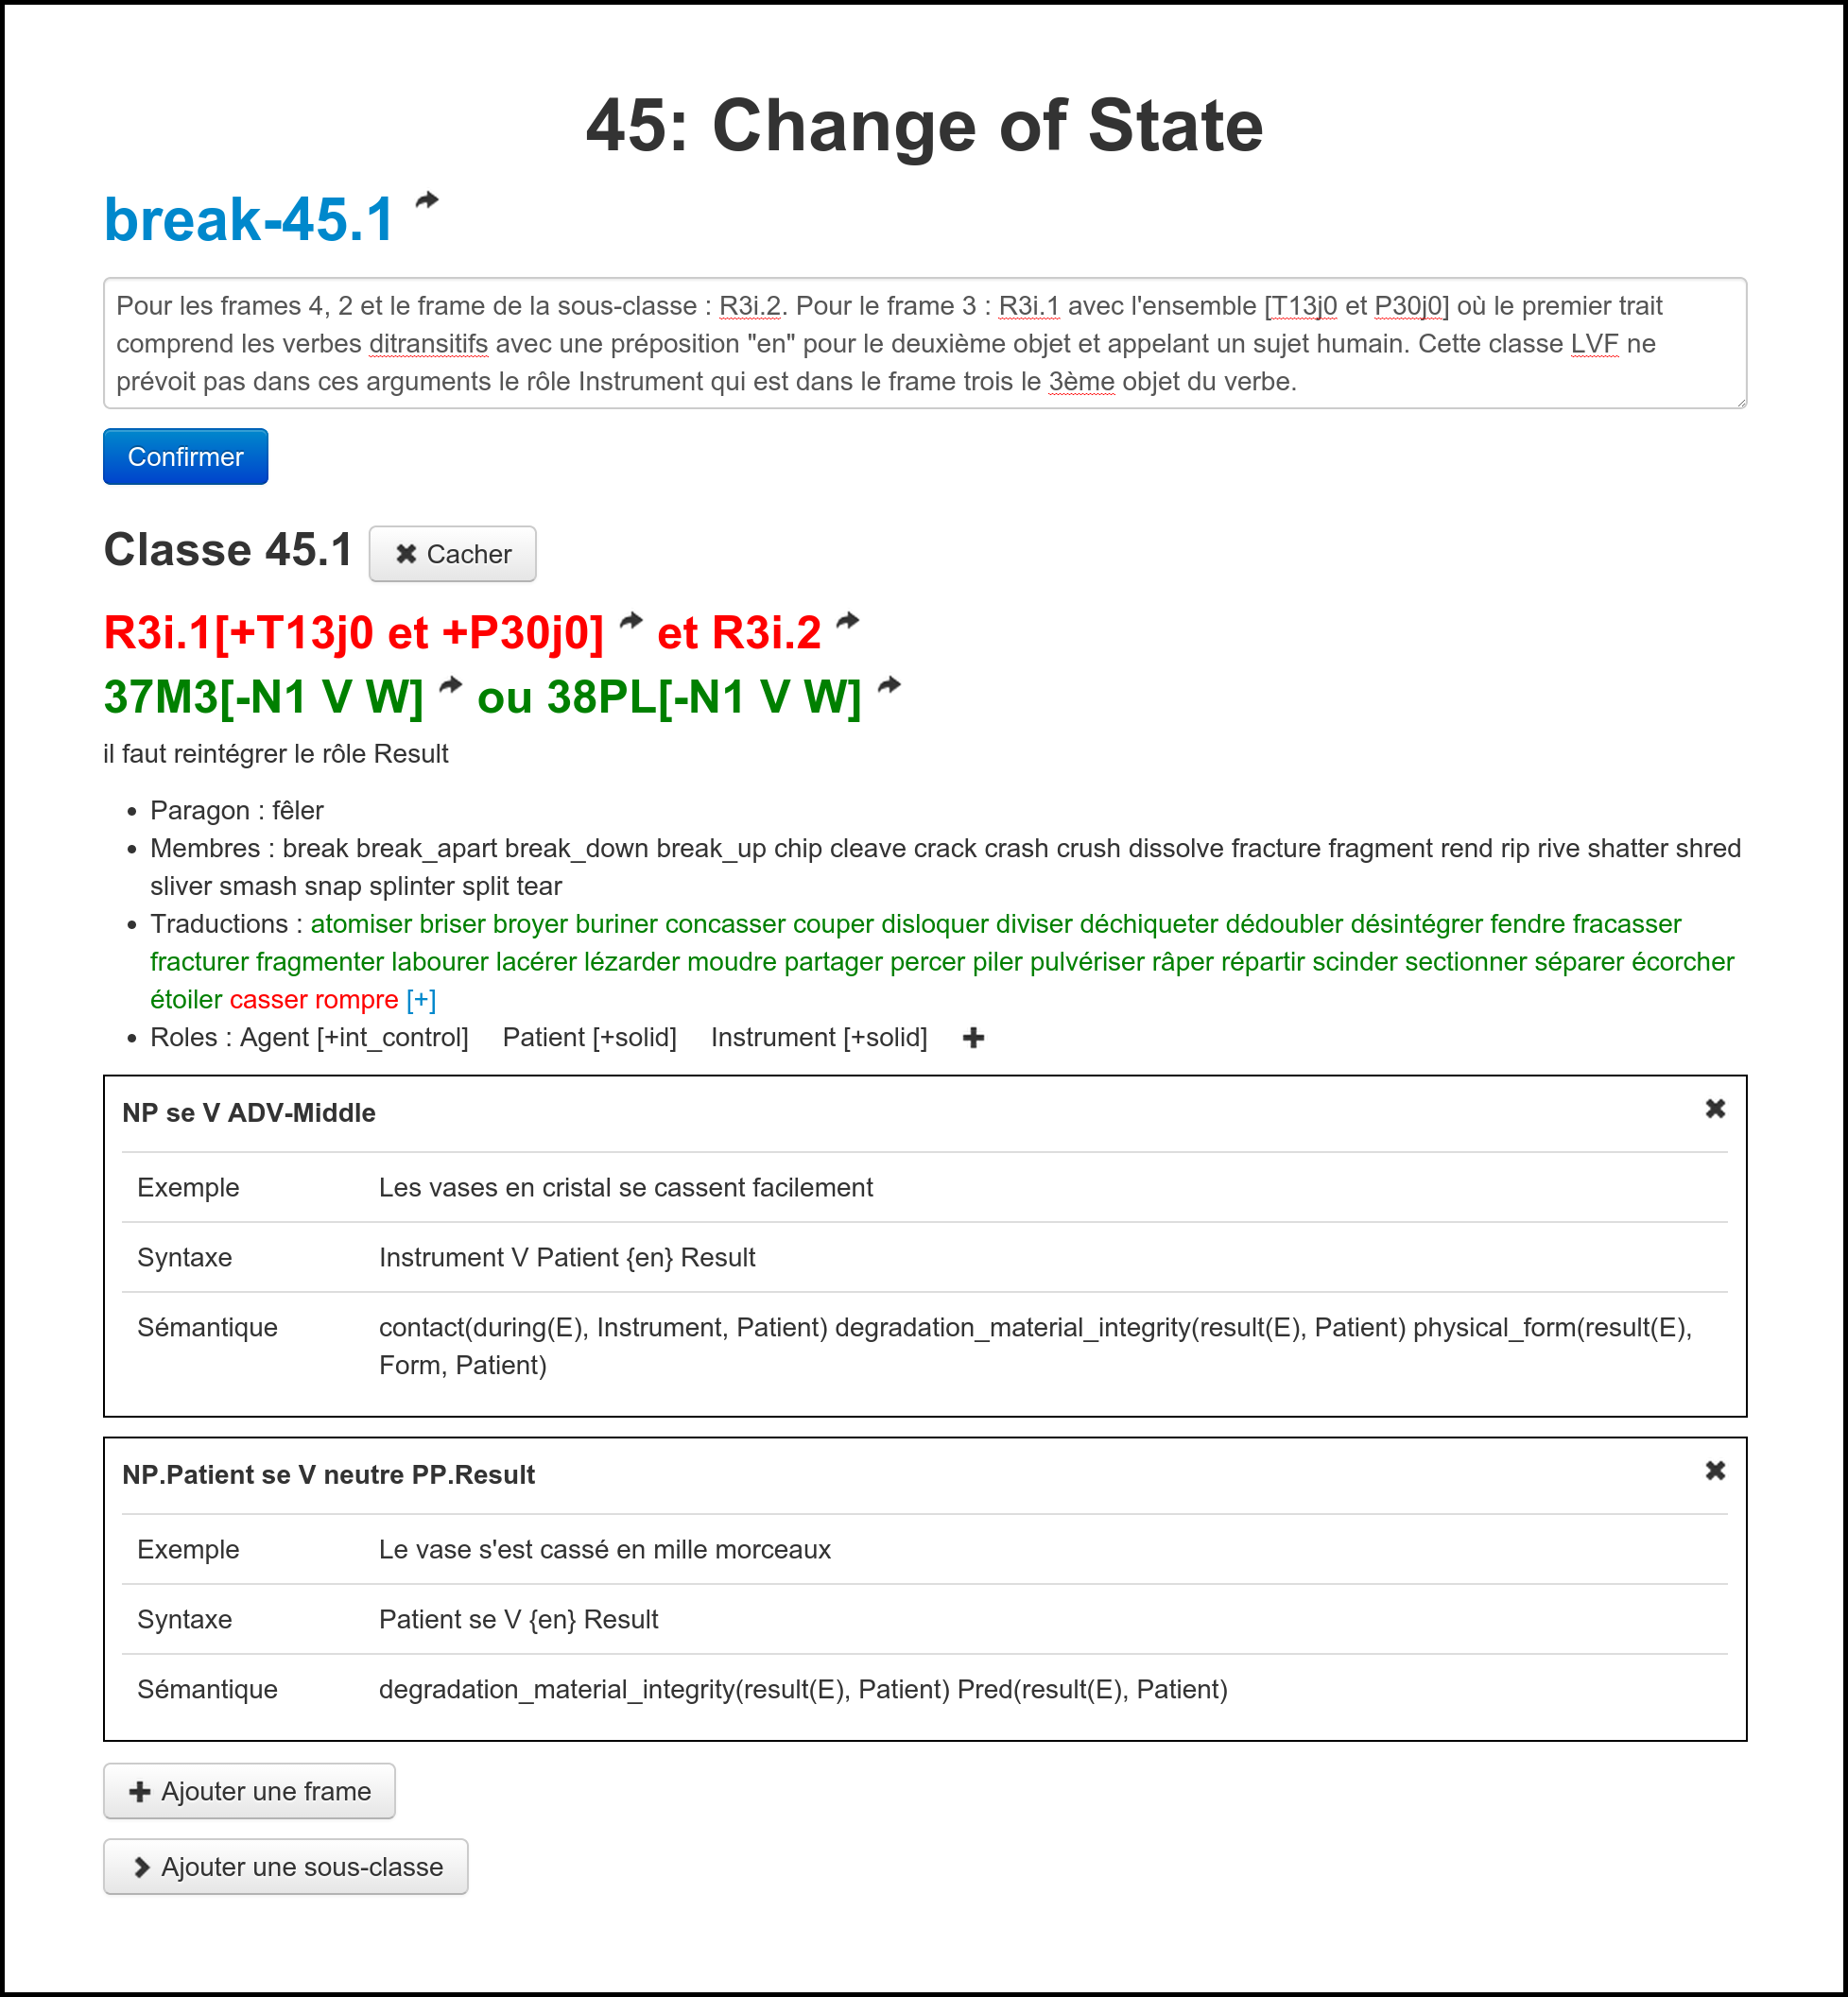
\includegraphics[width=\textwidth]{fig/tool_screenshot_2014-09-12.png}

    \caption{\label{tool}Interface web pour analyser et modifier \verbenet{}.
        Chaque frame peut être modifiée et les classes peuvent être
        réorganisées. Les traductions en violet apaprtiennent à l'intersection
        de \Clvf{}, \Clg{} et \Ltrad{} (section~\ref{first}), les traductions
        en rouge (respectivement en vert) uniquement à \Clvf{} et \Ltrad
        (respectivement uniquement à \Clg{} et \Ltrad{}). La description de
        {\color{blue}\texttt{break-45.1}} est en cours de modification : en cliquant sur
        'Confirmer', la modification sera prise en compte rapidement sans avoir
    à recharger la page pour éviter d'interrompre le travail lexicographique.}
\end{figure}


\subsection{Édition des correspondances}

Il est fréquent que les correspondances soient amenées à évoluer, et ce pour
trois raisons principales : la compréhension des classes anglaises peut
évoluer, la réorganisation peut demander des correspondances différentes, et il
peut être souhaitable d'affiner la correspondance en spécifiant certains
attributs de la classe française.

Il est donc possible de préciser qu'une colonne donnée doive être positive ou
négative. Deux exemples :
\begin{itemize}
    \item R3i.1[+T1308 et +P3000] ou R3i.1[+T1306 et +P3000] sélectionne tous
        les verbes de R3i.1 acceptant une construction pronominale (P3000) et
        une construction transitive direct à sujet humain, à objet non animé
        et a circonstant de modalité (T1306) ou instrumental, moyen (T1308).
    \item 4[+N1 se V de ce Qu P] sélectionne tous les verbes de la classe 
        4 ayant la valeur '+' à la colonne 'N1 se V de ce Qu P', ce qui
        signifie qu'ils acceptent cette forme.
\end{itemize}

Toutes ces correspondances sont validées avant d'être acceptées par le système,
ce qui est important pour éviter les erreurs, mais aussi pour s'assurer que le
traduction automatique des verbes fonctionne.

\subsection{Traduction des verbes en temps réel}

La première étape a permis de proposer des verbes français pour chacune des
classes du VerbNet anglais. Ces verbes français sont en fait maintenues en
temps réel par le système : à chaque modification des correspondances, les
verbes sont mis à jour : certains disparaissent, d'autres sont rajoutés. Cela
permet de vérifier instantanément la validité d'une correspondance du point de
vue des verbes français.

\subsection{Validation des verbes français}

La troisième étape, en cours parallèlement avec la deuxième, concerne la
validation des verbes. En cliquant sur un verbe français proposé à partir des
correspondances, ce verbe est soit validé, soit invalidé, soit remis à l'état
de simple proposition. Contrairement aux verbes proposés par correspondances,
les verbes validés ou invalidés ne sont jamais supprimés, même lorsque que la
correspondance change.

\subsection{Vérifications automatiques de la cohérence}

Petit à petit, différents outils sont ajoutés pour aider les lexicographes à
vérifier la cohérence de leur travail. Deux existent aujourd'hui.

Le premier identifie les verbes dupliqués au sein de la même super-classe de
Levin. En effet, bien qu'il soit naturel que le même lemme verbal soit présent
à plusieurs endroit de \verbenet{} pour des raisons de polysémie, les classes
de Levin regroupent des verbes sémantiquement proches : un verbe donné ne doit
être que dans une seule classe. Par ailleurs, quand un verbe peut exister à
différents endroits, c'est la classe la plus générale, souvent la première
qu'il faut choisir. Les utilisateurs connectés voient donc un encadré au début
de chaque classe de Levin leur indiquant quels verbes sont présents à plusieurs
endroit : il devient alors facile de valider/dévalider les verbes concernés.

Le second outil est l'index LADL (\url{http://verbenet.pradet.me/ladlindex/}).
L'objectif est de s'assurer qu'aucune classe des tables du LADL
(Lexique-Grammaire) majeure n'a été oubliée, et donc que le lexique couvre bien
l'ensemble des verbes du français. C'est en effet le cas : les seules classes
sans correspondance avec une classe \verbenet{} sont des classes résiduelles.
Cela réconforte l'idée selon laquelle \verbenet{} peut être vue comme une
réorganisation des tables du Lexique-Grammaire.

\subsection{Gestion des classes supprimées en anglais}

Lors d'une réorganisation, il est fréquent de ne plus avoir besoin d'une classe
en anglais. Nous traitons actuellement deux cas de figures possibles pour le
moment.

Premièrement, lorsqu'une sous-classe est supprimée, tous ses verbes anglais sont
automatiquement migrée vers sa classe mère, et les traductions des verbes
français sont mises à jour en fonction. C'est essentiel, étant donné que les
verbes les plus importants sont les plus polysémique et ceux acceptant le plus
de constructions : ils sont donc souvent dans les sous-classes.

Deuxièmement, lorsqu'une classe est simplement supprimée sans classe mère, ses
verbes sont théoriquement "perdus". Il est possible de transférer ces verbes
vers une autre classe plus appropriée, tout en gardant l'origine des verbes
anglais, au cas où cette opération devait être annulée. Ici aussi, les verbes
français sont ensuite mis à jour.

Un autre mécanisme sera nécessaire pour compléter l'ensemble de la
ressource : le mécanisme de répartition. En effet, une classe anglais est
parfois découpée en plusieurs classes français. Il faut alors, suivant les
correspondances vers les ressources français, placer les traductions
françaises vers l'une de ces classes. Plus généralement, il faut parfois
complètement réorganiser une classe, ce qui est le cas des verbes de changement
de possession ou des verbes de combinaison et de liaison. Dans ce cas, il faut
recréer entièrement la hiérarchie pour le français, puis il faut considérer
globalement les traductions de tous les verbes anglais, et placer chaque
traduction dans la sous-classe la plus appropriée.

\section*{Conclusion}

Nous avons présenté une méthode pour adapter la ressource syntaxico-sémantique
VerbNet vers une nouvelle langue. Cette méthode combine l'automatisation du
transfert de frames, la traduction automatique du lexique et une expertise
linguistique. Nous avons appliqué cette méthode au français et avons atteint un
point où cette ressource est validée et le travail systématique sur chaque
classe est en cours. Nous reconnaissons les différences qui existent entre les
langues : la structure de \verbenet{} n'est pas exactement celle de VerbNet.

% TODO exporter dans un format libre et mettre quelque part !

% TODO on doit connaître l'état de la ressource et le travail restant
